\chapter{Weyl Semimetalic Phase of $($TaSe$_4)_2$I}

$(\mathrm{TaSe}_4)_2\mathrm{I}$ is a quasi-one-dimensional crystal in space group 97 ($I422$). Viewing from the $z$ direction, $\mathrm{TaSe}_4$ chains are arranged in a checkerboard lattice in $xy$ plane (see figure~\ref{fig:tasesymmetry}). Each unit cell contains two $\mathrm{TaSe}_4$ chains (labeled by $\mu=\mathrm{I},\mathrm{II}$) and they are separated by the iodine (I) atoms. The low-energy electronic degrees of freedom can be approximated on each chain by a 1D model with two sublattice sites (labeled by $\tau=1,2$) in each unit cell. Despite having a body-centered tetragonal structure, in this paper, we represent the crystal in a primitive tetragonal structure generated by translations $T_x,T_y,T_z$ in the orthogonal directions, where the unit-cells are artificially enlarged. The translation symmetry is extended by body-centered translations $\hat{T}_{1/2}$ which interchange the two chain types and the two sublattices. In addition to lattice translations, the system also preserves time reversal symmetry $\hat{\mathcal{T}}$, the fourfold rotation symmetry $\hat{C}_{4z}^s$ about $z$-axis, and the twofold rotation symmetry $\hat{C}_{2x}$ about $x$-axis. 
 \begin{figure}
     \centering
     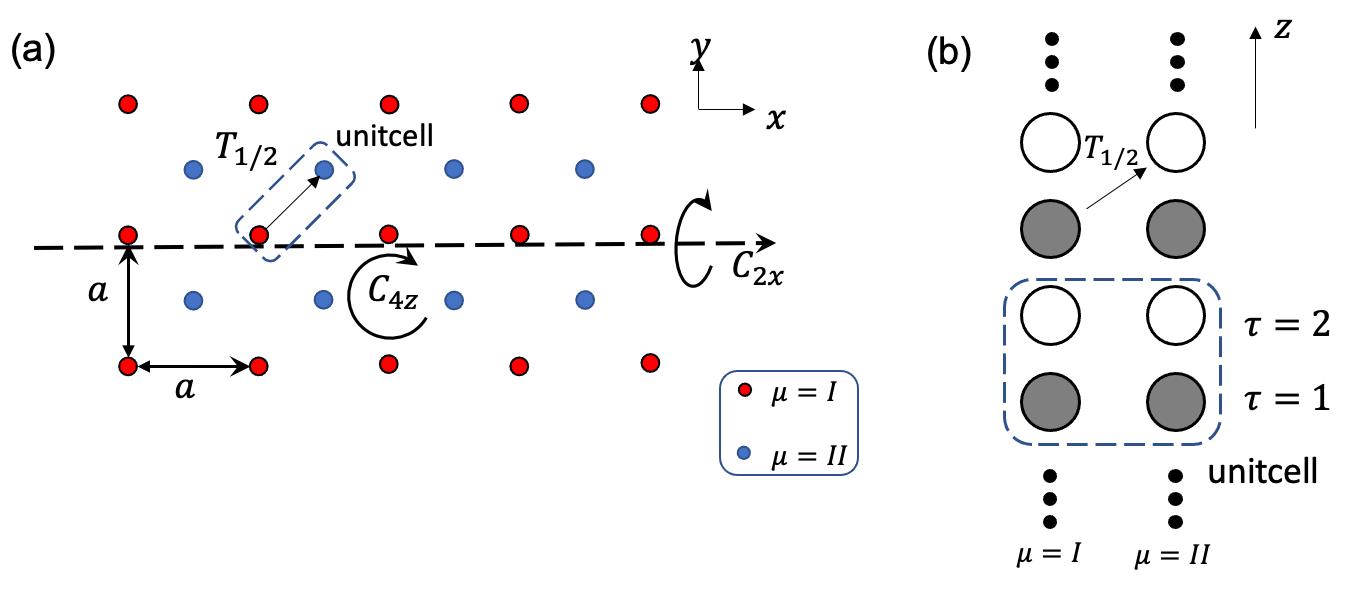
\includegraphics[width =\textwidth]{images/tasesymmetry.png}
     \caption{Symmetry of $(\mathrm{TaSe}_4)_2\mathrm{I}$.(a) Viewing from the z axis, each dot represent a  $\mathrm{TaSe}_4$ chains and they are aligned in a checkerboard lattice in $xy-$plane. Each unit cell contains two chains (labeled by red  and blue) connected by an body-centered translation $\hat{T}_{1/2}$. (b) Two chain $\mu=I$ and $\mu=II$ along z-axis. For each chain there are two sites inside unit cell represented by $\tau=1,2$. Each site also contains spin degree of freedom $s=\uparrow, \downarrow$.}
     \label{fig:tasesymmetry}
 \end{figure}



\section{The one-dimensional chain and its continuous approximation}

We consider a one-dimensional spinful chain with two sites $\tau_z=1,2$ per unit cell. Adjacent sites are separated by $c/2$ and the (artificially doubled) unit cell has the lattice constant $c$. 
The electron (annihilation) operators are ${\bf c}(z)=(c_{\uparrow1}(z),c_{\downarrow1}(z),c_{\uparrow2}(z),c_{\downarrow2}(z))^T$, where $z=mc$ represents the position of the $m^{\mathrm{th}}$ unit cell, for $m\in\mathbb{Z}$. The tight-binding Hamiltonian with nearest neighbour hopping is

\begin{align}
    \hat{H}_1&=-\frac{\hbar v}{c}\sum_z\sum_{s=\uparrow,\downarrow}\left(c_{s1}(z)^\dagger c_{s2}(z)+c_{s2}(z)^\dagger c_{s1}(z+c)+h.c.\right)\nonumber\\
    &\;\;\;-i\frac{\Delta_{SO}}{2}\sum_z\left(c_{\uparrow1}(z)^\dagger c_{\uparrow2}(z)+c_{\uparrow2}(z)^\dagger c_{\uparrow1}(z+c)-h.c.\right)\nonumber\\
    &\;\;\;+i\frac{\Delta_{SO}}{2}\sum_z\left(c_{\downarrow1}(z)^\dagger c_{\downarrow2}(z)+c_{\downarrow2}(z)^\dagger c_{\downarrow1}(z+c)-h.c.\right)\nonumber\\
    &=\int_{-\pi/c}^{\pi/c}\frac{cdk}{2\pi}{\bf c}(k_z)^\dagger H_1(k_z){\bf c}(k_z),\label{H1}
\end{align}
where $\frac{\hbar v}{c}$ is the nearest hopping between two sites and $\Delta_{SO}$ is the spin-orbital coupling between nearest neighbour. The Fourier transformation is defined by 
\begin{equation}
\begin{aligned}
     c_{s\tau}(k_z)=\sum_ze^{ik_zz}c_{s\tau}(z)\\ c_{s\tau}(z)=\int_{-\pi/c}^{\pi/c}\frac{cdk_z}{2\pi}e^{-ik_zz}c_{s\tau}(k_z)
\end{aligned}
\end{equation}
and the Bloch Hamiltonian is 
\begin{align}
H_1(k_z)=&\begin{pmatrix}
0&-\hbar v(1+e^{ik_zc})/c-i\Delta_{SO}s_z(1-e^{ik_zc})/2\\
h.c.&0\end{pmatrix}\nonumber\\
=&-\left[\frac{\hbar v}{c}\left(1+\cos(k_zc)\right)+\frac{\Delta_{SO}}{2}\sin(k_zc)s_z\right]\tau_x\\&+\left[\frac{\hbar v}{c}\sin(k_zc)+\frac{\Delta_{SO}}{2}\left(1-\cos(k_zc)\right)s_z\right]\tau_y.
\label{BlochH1}
\end{align}

For $0\lesssim\Delta_{SO}\ll\hbar v/c$ and Fermi energy $\epsilon_f\approx0$, the low-energy expansion near the Fermi momentum around $k_z=\pi/c+\delta k$ is 
\begin{align}
    H_1(\pi/c+\delta k)=\hbar vk_z\tau_y+\Delta_{SO}s_z\tau_y+O(\delta k^2).
\end{align}

The symmetry group is generated by 
\begin{align}
\begin{split}
    &\hat{T}_z{\bf c}(k_z)\hat{T}_z^{-1}=e^{-ik_zz}{\bf c}(k_z),\\&\hat{\mathcal{T}}{\bf c}(k_z)\hat{\mathcal{T}}^{-1}=is_y{\bf c}(-k_z)^\ast,\\&\hat{C}_{2x}{\bf c}(k_z)\hat{C}_{2x}^{-1}=e^{i(\pi/2)s_x}\tau_x{\bf c}(-k_z)=is_x\tau_x{\bf c}(-k_z)\\&\hat{C}^s_{4z}{\bf c}(k_z)\left(\hat{C}^s_{4z}\right)^{-1}=\begin{pmatrix}0&e^{i(\pi/4)s_z}\\e^{-ik_zc+i(\pi/4)s_z}&0\end{pmatrix}{\bf c}(k_z).
\end{split}\label{1Dchainsymm0}
\end{align} 
The single-body representations of the translation, time-reversal, $C_{2x}$ rotation and $C^s_{4z}$ screw symmetries are 
\begin{equation}
\begin{aligned}
    &T_z(k_z)=e^{-ik_zz},\\
    &\mathcal{T}=is_y\mathcal{K},\\
    &C_{2x}=is_x\tau_x,\\
    &C^s_{4z}(k_z)=\begin{pmatrix}0&e^{i(\pi/4)s_z}\\e^{-ik_zc+i(\pi/4)s_z}&0\end{pmatrix}.
\end{aligned}
\end{equation}
The symmetry operators obey the algebraic relations \begin{align}\begin{split}&\hat{\mathcal{T}}^2=(-1)^F,\quad[\hat{\mathcal{T}},\hat{T}_z]=[\hat{\mathcal{T}},\hat{C}_{2x}]=[\hat{\mathcal{T}},\hat{C}^s_{4z}]=0,\\&\hat{C}_{2x}\hat{T}_z\hat{C}_{2x}^{-1}=\hat{T}_z^{-1},\quad[\hat{T}_z,\hat{C}^s_{4z}]=0,\\&\hat{C}_{2x}^2=(-1)^F,\quad\hat{C}_{2x}\hat{C}^s_{4z}\hat{C}_{2x}^{-1}=\left(\hat{C}^s_{4z}\right)^{-1},\\&\left(\hat{C}^s_{4z}\right)^2=\hat{C}_{2z}\hat{T}_z,\quad\hat{C}_{2z}^2=(-1)^F\end{split}\end{align} where $(-1)^F$ is the fermion parity operator and $\hat{C}_{2z}{\bf c}(\delta k)\hat{C}_{2z}^{-1}=e^{i(\pi/2)s_z}{\bf c}(\delta k)=is_z{\bf c}(\delta k)$. These relations are consistent with the single-body representations \begin{align}
\begin{split}
&\mathcal{T}^2=-1,\quad\mathcal{T}:k_z\to-k_z,\\
& s_yC_{2x}^\ast s_y=C_{2x},\quad s_yC^s_{4z}(k_z)^\ast s_y=C^s_{4z}(-kz),\\
&C_{2x}:k_z\to-k_z,\quad C^s_{4z}:k_z\to k_z,\\
&C_{2x}^2=-1,\quad C_{2x}^{-1}C^s_{4z}(-k_z)C_{2x}=\left(C_{4z}(k_z)\right)^{-1},\\
&\left(C^s_{4z}(k_z)\right)^2=e^{-ik_zc}is_z.
\end{split}
\end{align} 

The Hamiltonian is symmetric under these symmetries. \begin{align}
s_yH_1(k_z)^\ast s_y=H_1(-k_z),\\
C_{2x}^{-1}H_1(k_z)C_{2x}=H_1(-k_z),\\
C^s_{4z}(k_z)^{-1}H_1(k_z)C^s_{4z}(k_z)=H_1(k_z).
\label{1dchainsymm1}
\end{align} 
$H_1$ is also the most general tight-binding model with onsite and nearest neighbor tunnelings allowed by the symmetries up to a constant. The 1D chain has an emergent half-translation symmetry $[\hat{H}^1,\hat{T}_{c/2}]=0$, where \begin{gather}\hat{T}_{c/2}{\bf c}(k_z)\hat{T}_{c/2}^{-1}=T_{c/2}(k_z){\bf c}(k_z),\quad T_{c/2}(k_z)=\begin{pmatrix}0&1\\e^{-ik_zc}&0\end{pmatrix}\label{halfTc}\\T_{c/2}(k_z)^\dagger H_1(k_z)T_{c/2}(k_z)=H_1(k_z).\nonumber\end{gather} This is not an actual microscopic symmetry of the 1D chain and can be broken by next nearest neighbor tunnelings. 

The 1D chain model has the low-energy continuous approximation around the Fermi energy $\epsilon_f=0$ 
\begin{align}
    \hat{H}_c&=\int_{-L/2}^{L/2}dz\boldsymbol\psi(z)^\dagger\left(-i\hbar v\tau_y\partial_z+\Delta_{SO}s_z\tau_y\right)\boldsymbol\psi(z)\\
    &=\sum_k\boldsymbol\psi_k^\daggerH_c(k)\boldsymbol\psi_k\nonumber\\
    H_c(k)&=\hbar vk\tau_y+\Delta_{SO}s_z\tau_y
\label{H1cont}
\end{align}

where $z$ is now a continuous variable compactified on a circle with circumference $L\to\infty$ and momentum $k$ is discretized in increments of $2\pi/L$. The Dirac fermions $\boldsymbol\psi=(\psi_{\uparrow1},\psi_{\downarrow1},\psi_{\uparrow2},\psi_{\downarrow2})^T$ obey the anti-commutation relations $\{\psi^{s\tau}(z),\psi^{s'\tau'}(z')\}=\{\psi^{s\tau}_k,\psi^{s'\tau'}_{k'}\}=0$, $\{\psi^{s\tau}(z),\psi^{s'\tau'}(z')^\dagger\}=\delta^{ss'}\delta^{\tau\tau'}\delta(z-z')$ and $\{\psi^{s\tau}_k,{\psi^{s'\tau'}_{k'}}^\dagger\}=\delta^{ss'}\delta^{\tau\tau'}\delta_{k,k'}$. The Fourier transformation is defined by \begin{gather}\psi^{s\tau}_k=\int_{-L/2}^{L/2}\frac{dz}{\sqrt{L}}e^{ikz}\psi^{s\tau}(z),\quad\psi^{s\tau}(z)=\frac{1}{\sqrt{L}}\sum_ke^{-ikz}\psi^{s\tau}_k.\end{gather} The continuous and lattice fermions are related by the identification \begin{align}\psi^{s\tau}_k=c_{s\tau}(\pi/c+k),\quad\mbox{for $|kc|\ll1$}.\end{align}

The symmetry operations are identical to the lattice case \eqref{1Dchainsymm0} except for the lattice $C_4^s$ screw symmetry, which becomes a symmorphic $C_4$ rotation in the continuous approximation. \begin{align}\begin{split}&\hat{\mathcal{T}}\boldsymbol\psi(k)\hat{\mathcal{T}}^{-1}=is_y\boldsymbol\psi(-k)^\ast,\\&\hat{C}_{2x}\boldsymbol\psi(k)\hat{C}_{2x}^{-1}=e^{i(\pi/2)s_x}\tau_x\boldsymbol\psi(-k)=is_x\tau_x(-k)\\&\hat{C}_{4z}\boldsymbol\psi(k)\hat{C}_{4z}^{-1}=e^{i(\pi/4)s_z}i\tau_y\boldsymbol\psi(k).\end{split}\end{align} The single-body symmetry representations are \begin{align}\mathcal{T}=is_y\mathcal{K},\quad C_{2x}=is_x\tau_x,\quad C_{4z}=e^{i(\pi/4)s_z}i\tau_y.\end{align} The discrete lattice translation symmetry emerges as a continuous symmetry $\hat{T}_z\boldsymbol\psi(k)\hat{T}_z^{-1}=e^{-ikz}\boldsymbol\psi(k)$, where $z$ is now continuous. In particular, the lattice $C^s_{4z}$ screw symmetry becomes the symmorphic $C_{4z}$ rotation in the continuous approximation when composed with the emergent half-translation $T_{c/2}$. \begin{align}C^s_{4z}(k_z)&=e^{i(\pi/4)s_z}\begin{pmatrix}0&1\\e^{-ik_zc}&0\end{pmatrix}=e^{i(\pi/4)s_z}\begin{pmatrix}0&1\\e^{-i(\pi/c+k)c}&0\end{pmatrix}\nonumber\\&\approx e^{-ik_zc}\begin{pmatrix}0&1\\-1&0\end{pmatrix}=e^{-ik_zc}i\tau_y=C_{4z},\quad\mbox{when $|kc|\ll1$}.\end{align} It should be noted that the continuous approximation \eqref{H1cont} is actually not symmetric under the lattice $C^s_{4z}$ screw and the linear Hamiltonian \eqref{H1cont} does not obey \eqref{1dchainsymm1}. Instead the single body Hamiltonian obeys the new symmetries, \begin{align}s_yH_1(k)^\ast s_y=H_1(-k),\quad C_{2x}^{-1}H_1(k)C_{2x}=H_1(-k),\quad C_{4z}^{-1}H_1(k_z)C_{4z}=H_1(k).\end{align}






\section{The three-dimensional body-centered model}

\subsection{The coupled-chain tight-binding lattice model}
The coupled-chain model is constructed by a 3D array of chains parallel to the $z$-direction and occupying the checkered board lattice along the $xy$ plane. The fermion (annihilation) operators are ${\bf c}_\mu({\bf r})$, where ${\bf r}=(x,y,z)=a(m_x{\bf e}_x+m_y{\bf e}_y)+cm_z{\bf e}_z$ represents the unit cell on the square lattice for $m_{x,y,z}\in\mathbb{Z}$, and $\mu=I,II$ labels the two chains (represented by the red and blue dots in figure~\ref{fig:tasesymmetry}) in the same unit cell displaced by $(\frac{1}{2}\frac{1}{2}\frac{1}{2})=a(m_x{\bf e}_x+m_y{\bf e}_y)/2+c{\bf e}_z/2$. We group the 2 wires per unit cell into the 8-dimensional column vector ${\bf c}({\bf r},\delta k)=({\bf c}_{\Rmnum{1}}({\bf r},\delta k),{\bf c}_{II}({\bf r},\delta k))^T$. The coupled wire model consists of the intra-wire kinetic Hamiltonian $\hat{H}_1$ defined in \eqref{H1} and \eqref{BlochH1} and nearest neighbor electron tunneling. 
\begin{align}\hat{H}&=\hat{H}_1+\delta\hat{H}\label{CWM1}\\\hat{H}_1&=\sum_{x,y}\int_{-\pi/c}^{\pi/c}\frac{cdk_z}{2\pi}\sum_{\mu=I,II}{\bf c}_\mu(x,y,k_z)^\dagger H_1(k_z){\bf c}_\mu(x,y,k_z),\nonumber\\\delta\hat{H}&=\sum_{x,y}\frac{cdk_z}{2\pi}\left[{\bf c}_{II}(x,y,k_z)^\dagger t_a+{\bf c}_{II}(x-a,y,k_z)^\dagger t_b\right.\nonumber\\&\quad\quad\quad\quad\left.+{\bf c}_{II}(x,y-a,k_z)^\dagger t_c+{\bf c}_{II}(x-a,y-a,k_z)^\dagger t_d\right]{\bf c}_{\Rmnum{1}}(x,y,k_z)+h.c.\nonumber\end{align} where the single-body tunneling amplitudes $t_{a,b,c,d}$ are $4\times4$ matrices. From figure~\ref{fig:tightbinding}, the nearest neighbor tunnelings only couple sites with the same $\tau$, and therefore the amplitudes are block diagonal \begin{align}t=t^1\oplus t^2=\begin{pmatrix}t^1&0\\0&t^2\end{pmatrix}\label{chainhoppings}\end{align} where $t^\tau=(t^\tau_{ss'})_{2\times2}$ are matrices acting on spins.

We define the Fourier transform \begin{align}c_{s\tau\mu}({\bf k})=\sum_{\bf r}e^{i{\bf k}\cdot{\bf r}}c_{s\tau\mu}({\bf r}),\quad c_{s\tau\mu}({\bf r})=\int_{BZ}\frac{a^2cdk_xdk_yd_z}{(2\pi)^3}e^{-i{\bf k}\cdot{\bf r}}c_{s\tau\mu}({\bf k})\end{align} so that $\hat{T}_{\bf r}{\bf c}({\bf r}')\hat{T}_{\bf r}^{-1}={\bf c}({\bf r}+{\bf r}')$ and $\hat{T}_{\bf r}{\bf c}({\bf k})\hat{T}_{\bf r}^{-1}=e^{-i{\bf k}\cdot{\bf r}}{\bf c}({\bf k})$. Here $BZ$ is the Brillouin zone containing lattice momentum ${\bf k}=k_x{\bf e}_x+k_y{\bf e}_y+k_z{\bf e}_z$ where $k_x,k_y\in[-\pi/a,\pi/a]$ and $k_z\in[-\pi/c,\pi/c]$. The coupled chain model \eqref{CWM1} becomes \begin{align}\begin{split}\hat{H}&=\hat{H}_1+\delta\hat{H}=\int_{BZ}\frac{a^2cdk_xdk_ydk_z}{(2\pi)^3}{\bf c}({\bf k})^\dagger H({\bf k}){\bf c}({\bf k})\\\hat{H}_1&=\int_{BZ}\frac{a^2cdk_xdk_ydk_z}{(2\pi)^3}\sum_{\mu=I,II}{\bf c}_\mu({\bf k})^\dagger H_1(k_z){\bf c}_\mu({\bf k}),\\\delta\hat{H}&=\int_{BZ}\frac{a^2cdk_xdk_ydk_z}{(2\pi)^3}{\bf c}_{II}({\bf k})^\dagger\left[t_a+t_be^{-ik_xa}+t_ce^{-ik_ya}+t_de^{-i(k_x+k_y)a}\right]{\bf c}_{\Rmnum{1}}({\bf k},\delta k)+h.c..\end{split}\label{CWM2}\end{align} The Bloch Hamiltonian is \begin{align}H({\bf k},\delta k)&=\begin{pmatrix}H_1(k_z)&t_a^\dagger+t_b^\dagger e^{ik_xa}+t_c^\dagger e^{ik_ya}+t_d^\dagger e^{i(k_x+k_y)a}\\t_a+t_be^{-ik_xa}+t_ce^{-ik_ya}+t_de^{-i(k_x+k_y)a}&H_1(\delta k)\end{pmatrix}.\label{Blochansatz1}\end{align} where $H_1(k_z)$ was derived in \eqref{BlochH1}. Here the on-chain kinetic Hamiltonian are identical for the 2 chains $\mu=I,II$ because of the emergent half-translation symmetry in \eqref{halfTc}. In general, the 2 chains are shifted by $c/2$ in the $z$-direction and therefore should be distinguished by $\hat{H}^{II}_1=\hat{T}_{c/2}\hat{H}^I_1\hat{T}_{c/2}^\dagger$.

The body-centered lattice structure is recovered by the addition of the translation symmetry $T_{(\frac{1}{2}\frac{1}{2}\frac{1}{2})}=T_{1/2}$ (see figure~\ref{fig:tightbinding}). 
\begin{align}
\begin{split}&\hat{T}_{1/2}c_{s,1,I}({\bf r})\hat{T}_{1/2}^{-1}=c_{s,2,II}({\bf r}),\quad\hat{T}_{1/2}c_{s,2,I}({\bf r})\hat{T}_{1/2}^{-1}=c_{s,1,II}({\bf r}+c{\bf e}_z),\\&\hat{T}_{1/2}c_{s,1,II}({\bf r})\hat{T}_{1/2}^{-1}=c_{s,2,I}({\bf r}+a{\bf e}_x+a{\bf e}_y),\\
&\hat{T}_{1/2}c_{s,2,II}({\bf r})\hat{T}_{1/2}^{-1}=c_{s,1,I}({\bf r}+a{\bf e}_x+a{\bf e}_y+c{\bf e}_z),
\end{split}
\label{thalf3d}
\end{align} 
or equivalently, in Fourier space, 
\begin{align}
\hat{T}_{1/2}{\bf c}({\bf k})\hat{T}_{1/2}^{-1}&=T_{1/2}({\bf k}){\bf c}({\bf k}),\\
T_{1/2}({\bf k})=&
\begin{pmatrix}
0&1\\
e^{-ik_zc}&0
\end{pmatrix}
\otimes
\begin{pmatrix}
0&1\\
e^{-i(k_x+k_y)a}&0
\end{pmatrix}\\
=&T_{1/2}^\tau(k_z)T_{1/2}^\mu(k_x,k_y)\nonumber\\
=&e^{-i(k_x+k_y)a/2-ik_zc/2}\left[\cos\left(\frac{k_zc}{2}\right)\tau_x-\sin\left(\frac{k_zc}{2}\right)\tau_y\right]\\
&\times\left[\cos\left(\frac{(k_x+k_y)a}{2}\right)\mu_x-\sin\left(\frac{(k_x+k_y)a}{2}\right)\mu_y\right].\nonumber\end{align} The matrix $T_{1/2}^\tau(k_z)$ is exactly the single-body representation of the emergent half-translation matrix $T_{c/2}(k_z)$ defined in \eqref{halfTc}. The body-centered translation squares to $\hat{T}_{1/2}^2=\hat{T}_{(111)}$ and therefore its single-body representation obey $T_{1/2}({\bf k})^2=e^{-i{\bf k}.(a{\bf e}_x+a{\bf e}_y+c{\bf e}_z)}$. The body-centered symmetry $T_{1/2}({\bf k})^\dagger H({\bf k})T_{1/2}({\bf k})=H({\bf k},\delta k)$ requires \begin{gather}%t_a+t_be^{-ik_xa}+t_ce^{-ik_ya}+t_de^{-i(k_x+k_y)a}=e^{-i(k_x+k_y)a}T_{1/2}^\tau(k_z)^\dagger\left(t_a^\dagger+t_b^\dagger e^{ik_xa}+t_c^\dagger e^{ik_ya}+t_d^\dagger e^{i(k_x+k_y)a}\right)T_{1/2}^\tau(k_z)\nonumber\\\Leftrightarrow\quad
t_a^1=(t_d^2)^\dagger,\quad t_a^2=(t_d^1)^\dagger,\quad t_b^1=(t_c^2)^\dagger,\quad t_b^2=(t_c^1)^\dagger.\label{BCsymm}\end{gather} The time-reversal symmetry operator is represented by the anti-unitary transformation \begin{align}\hat{\mathcal{T}}\left[{\bf a}\cdot{\bf c}({\bf r})\right]\hat{\mathcal{T}}^{-1}=is_y{\bf a}^\ast\cdot{\bf c}({\bf r}),\quad\hat{\mathcal{T}}\left[{\bf a}\cdot{\bf c}({\bf k})\right]\hat{\mathcal{T}}^{-1}=is_y{\bf a}^\ast\cdot{\bf c}(-{\bf k}).\end{align} The single-body representation of the time-reversal operator is $\mathcal{T}=is_y\mathcal{K}$ that squares to $\mathcal{T}^2=-1$ because $\hat{\mathcal{T}}^2=(-1)^F$. The commutation relation $[\hat{\mathcal{T}},\hat{T}_{1/2}]=0$ is consistent with the algebraic relation \begin{align}\mathcal{T}T_{1/2}({\bf k})\mathcal{T}^{-1}=T_{1/2}(-{\bf k})\end{align} between the single-body matrix representations. The time-reversal symmetry $s_yH(-{\bf k},-\delta k)^\ast s_y=H(-{\bf k},-\delta k)$ requires \begin{align}s_yt_i^\ast s_y=t_i,\quad\mbox{for $i=a,b,c,d$}.\label{TRsymm}\end{align} 

The $C_{2x}$ symmetry operates according to 
\begin{align}
\hat{C}_{2x}{\bf c}_{\Rmnum{1}}(x,y,z)\hat{C}_{2x}^{-1}=is_x\tau_x{\bf c}_{\Rmnum{1}}(x,-y,-z),\\
\hat{C}_{2x}{\bf c}_{II}(x,y,z)\hat{C}_{2x}^{-1}=is_x\tau_x{\bf c}_{II}(x,-y-a,-z),
\end{align}
or equivalently, in Fourier space, 
\begin{align}
\hat{C}_{2x}{\bf c}({\bf k})\hat{C}_{2x}^{-1}=C_{2x}({\bf k}){\bf c}(r_{2x}{\bf k})&,\quad C_{2x}({\bf k})=is_x\tau_x
\begin{pmatrix}
1 & 0\\
0 & e^{-ik_ya}
\end{pmatrix}\\
r_{2x}:(k_x,k_y,k_z)&\to(k_x,-k_y,-k_z).
\end{align}
The algebraic relations $\hat{C}_{2x}^2=(-1)^F$, $[\hat{\mathcal{T}},\hat{C}_{2x}]=0$ and $\hat{C}_{2x}\hat{T}_{1/2}=\hat{T}_{-a{\bf e}_y-c{\bf e}_z}\hat{T}_{1/2}\hat{C}_{2x}$ are consistent with the single-body matrix representations 
\begin{gather}
C_{2x}({\bf k})C_{2x}(r_{2x}{\bf k})=-1,\quad\mathcal{T}C_{2x}({\bf k})\mathcal{T}^{-1}=C_{2x}(-{\bf k}),\nonumber\\T_{1/2}({\bf k})C_{2x}({\bf k})=e^{-i{\bf k}\cdot(a{\bf e}_y+c{\bf e}_z)}C_{2x}({\bf k})T_{1/2}(r_{2x}{\bf k}).
\end{gather} 
The $C_{2x}$ symmetry $C_{2x}({\bf k})^\dagger H({\bf k})C_{2x}({\bf k})=H(r_{2x}{\bf k})$ requires 
\begin{align}
t_a=s_x\tau_xt_cs_x\tau_x,\quad t_b=s_x\tau_xt_ds_x\tau_x.\label{C2xsymm}
\end{align} 

The $C^s_{4z}$ screw symmetry operates according to \begin{align}
\begin{split}&\hat{C}^s_{4z}{\bf c}_{\Rmnum{1}}(x,y,k_z)(\hat{C}^s_{4z})^{-1}=e^{i(\pi/4)s_z}T_{c/2}(k_z){\bf c}_{\Rmnum{1}}(-y,x,k_z),\\&\hat{C}^s_{4z}{\bf c}_{II}(x,y,k_z)(\hat{C}^s_{4z})^{-1}=e^{i(\pi/4)s_z}T_{c/2}(k_z){\bf c}_{II}(-y-a,x,k_z),
\end{split}
\end{align} or equivalently, in Fourier space, \begin{gather}\hat{C}^s_{4z}{\bf c}({\bf k})(\hat{C}^s_{4z})^{-1}=C^s_{4z}({\bf k}){\bf c}(r_{4z}{\bf k}),\\C^s_{4z}({\bf k})=e^{i(\pi/4)s_z}T_{c/2}(k_z)\begin{pmatrix}1&0\\0&e^{-ik_ya}\end{pmatrix},\quad r_{4z}:(k_x,k_y,k_z)\to(-k_y,k_x,k_z),\nonumber\label{C4zssymm}\end{gather} where $T_{c/2}(k_z)$ was defined in \eqref{halfTc} and act on the $\tau$ degree of freedom. The screw symmetry squares to $(\hat{C}^s_{4z})^2=\hat{C}_{2z}\hat{T}_{c{\bf e}_z}$, where $\hat{T}_{c{\bf e}_z}\leftrightarrow e^{-ik_zc}$ is the primitive $z$ translation, and $\hat{C}_{2z}$ is the symmorphic twofold rotation along the $\mu=I$ chain \begin{gather}
\hat{C}_{2z}{\bf c}_{\Rmnum{1}}(x,y,k_z)\hat{C}_{2z}^{-1}=is_z{\bf c}_{\Rmnum{1}}(-x,-y,k_z),\\
\hat{C}_{2z}{\bf c}_{II}(x,y,k_z)\hat{C}_{2z}^{-1}=is_z{\bf c}_{II}(-x-a,-y-a,k_z)\nonumber\\
\hat{C}_{2z}{\bf c}({\bf k})\hat{C}_{2z}^{-1}=C_{2z}({\bf k}){\bf c}(r_{2z}{\bf k}),\quad C_{2z}({\bf k})=is_z
\begin{pmatrix}
1&0\\
0&e^{-i(k_x+k_y)a}
\end{pmatrix},\quad r_{2z}=r^2_{4z},\\C^s({\bf k})C^s_{4z}(r_{4z}{\bf k})=e^{-ik_zc}C_{2z}({\bf k}).\nonumber\end{gather} Moreover, the $\hat{C}^s_{4z}$ screw symmetry can be combined with the body-centered translation $\hat{T}_{1/2}$ to form a symmorphic fourfold rotation $\hat{C}_{4z}=\hat{C}^s_{4z}\hat{T}_{1/2}\hat{T}_{-c{\bf e}_z}$, where 
\begin{gather}
\hat{C}_{4z}{\bf c}_{\Rmnum{1}}(x,y,k_z)\hat{C}_{4z}^{-1}=e^{i(\pi/4)s_z}{\bf c}_{II}(-y-a,x,k_z),\\
\hat{C}_{4z}{\bf c}_{II}(x,y,k_z)\hat{C}_{4z}^{-1}=e^{i(\pi/4)s_z}{\bf c}_{\Rmnum{1}}(-y-a,x+a,k_z),\nonumber\\
\hat{C}_{4z}{\bf c}({\bf k})\hat{C}_{4z}^{-1}=C_{4z}({\bf k}){\bf c}(r_{4z}{\bf k}),\quad C_{4z}({\bf k})=e^{i(\pi/4)s_z}\begin{pmatrix}0&e^{-ik_ya}\\e^{-i(k_x+k_y)a}&0\end{pmatrix},\\C_{4z}({\bf k})C_{4z}(r_{4z}{\bf k})=e^{-ik_xa}C_{2z}({\bf k}).\nonumber\end{gather} In addition, the fourfold rotation obey the symmetry relations with time-reversal, body-centered translation and twofold rotation \begin{align}[\hat{\mathcal{T}},\hat{C}_{4z}]=0,\quad\hat{C}_{4z}\hat{T}_{1/2}\hat{C}_{4z}^{-1}=\hat{T}_{-a{\bf e}_x}\hat{T}_{1/2},\quad\hat{C}_{2x}\hat{C}_{4z}\hat{C}_{2x}^{-1}=\hat{C}_{4z}^{-1}.\end{align} These relations are consistent with the single-body matrix representations \begin{gather}\begin{split}&\mathcal{T}C_{4z}({\bf k})\mathcal{T}^{-1}=C_{4z}(-{\bf k}),\quad T_{1/2}({\bf k})C_{4z}({\bf k})=C_{4z}({\bf k})T_{1/2}(r_{4z}{\bf k})e^{-ik_ya},\\&C_{4z}({\bf k})C_{2x}(r_{4z}{\bf k})=C_{2x}({\bf k})C_{4z}(r_{4z}^{-1}r_{2x}{\bf k})^{-1}.\end{split}\end{gather} The $C_{4z}$ symmetry \begin{align}C_{4z}({\bf k})^\dagger H({\bf k})C_{4z}({\bf k})=H(r_{4z}{\bf k})\end{align} rotates the tunneling amplitudes \begin{align}t_a=e^{-i(\pi/4)s_z}t_b^\dagger e^{i(\pi/4)s_z}=s_zt_ds_z=e^{i(\pi/4)s_z}t_c^\dagger e^{-i(\pi/4)s_z}.\label{C4zsymm}\end{align}

The body-centered and $C_{2x}$ symmetries \eqref{BCsymm} and \eqref{C2xsymm} restrict the tunneling amplitudes \eqref{chainhoppings} into two $2\times2$ matrices $t^\tau$, for $\tau=1,2$, 
\begin{align}
t_a=\begin{pmatrix}t^1&0\\0&t^2\end{pmatrix},\quad t_b=\begin{pmatrix}s_x(t^1)^\dagger s_x&0\\0&s_x(t^2)^\dagger s_x\end{pmatrix},\\
t_c=\begin{pmatrix}s_xt^2s_x&0\\0&s_xt^1s_x\end{pmatrix},\quad t_d=\begin{pmatrix}(t^2)^\dagger&0\\0&(t^1)^\dagger\end{pmatrix}.\end{align} The time-reversal and $C_{4z}$ screw symmetries \eqref{TRsymm} and \eqref{C4zsymm} further require \begin{align}s_y(t^\tau)^\ast s_y=t^\tau,\quad t^1=s_nt^1s_n=s_z(t^2)^\dagger s_z,\quad\mbox{where }s_n=(s_x+s_y)/\sqrt{2}.\label{nnhoppingt} \end{align} A general symmetry-preserving tunneling amplitude is generated by the linear combinations of 2 terms \begin{gather}t^1=t^2=p\mathbb{I}+iqs_n,\quad\mbox{where $p,q\in\mathbb{R}$.}\nonumber\\t_a=t_d^\dagger=p+iqs_n,\quad t_c=t_b^\dagger=p+iqs_n^T.\end{gather} Like the 1D case, here a half-translation $T_{c/2}$ along the $z$-direction emerges in the nearest neighbor tunneling approximation because the tunneling amplitudes $t_{a,b,c,d}$ act trivially on the $\tau$ degrees of freedom. 

{\color{red} p is not comparable with the intra chain coupling
q is not supported by symmetry.}

\subsection{The simple cubic lattice model}
Here we unwrap the previous coupled-chain tight-binding model on a tetragonal lattice with one site per unit cell. The reduction of the unit cell is a result of the extension of the body-centered translation $T_{(\frac{1}{2}\frac{1}{2}\frac{1}{2})}$ and the emergent half-translation $T_{(00\frac{1}{2})}$. The primitive translations of the tetragonal lattice are ${\bf a}_1=a({\bf e}_x+{\bf e}_y)/2$, ${\bf a}_2=a(-{\bf e}_x+{\bf e}_y)/2$ and ${\bf a}_3=c{\bf e}_z/2$. The primitive reciprocal lattice vectors are ${\bf a}_1=2\pi({\bf e}_x+{\bf e}_y)/a$, ${\bf b}_2=2\pi(-{\bf e}_x+{\bf e}_y)/a$ and ${\bf b}_3=4\pi{\bf e}_z/c$. The tight-binding Hamiltonian is \begin{align}\hat{H}&=\int_{BZ}\frac{(a^2c/4)d^3{\bf k}}{(2\pi)^3}\sum_{s,s'=\uparrow,\downarrow}c_s({\bf k})^\dagger H_{ss'}({\bf k})c_{s'}({\bf k})\label{threedimensional} ,\\H({\bf k})&=\left[-\frac{2\hbar v}{c}\cos({\bf k}\cdot{\bf a}_3)+2p\left(\cos({\bf k}\cdot{\bf a}_1)+\cos({\bf k}\cdot{\bf a}_2)\right)\right]\mathbb{I}\nonumber\\&\;\;\;-2q\sin({\bf k}\cdot{\bf a}_1)s_n+2q\sin({\bf k}\cdot{\bf a}_2)s_n^T-2\Delta_{SO}\sin({\bf k}\cdot{\bf a}_3)s_z\nonumber\end{align}



\subsection{Tight-binding model of Weyl semimetal phase}
\begin{figure}[h]
    \centering
    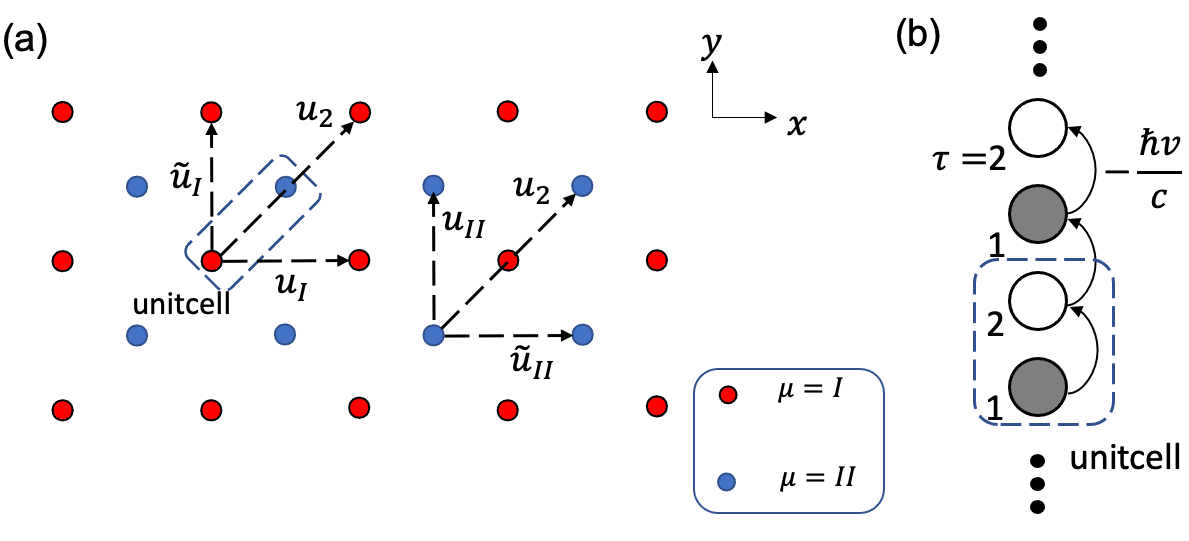
\includegraphics[width=\textwidth]{images/tightbindingWeyl.png}
    \caption{Tight-binding model of $(\mathrm{TaSe}_4)_2\mathrm{I}$ Weyl semimetal phase. (a) Inter-unit cell hopping $\hat{H}_2$ and $\hat{H}_3$ terms. (b) The intra-chain nearest neighbour tunneling $\hat{H}_1$ term.}
    \label{fig:tightbinding}
\end{figure}

We introduce a 8 band spinful tight binding model capturing the Weyl semimetal phase of $(\mathrm{TaSe}_4)_2\mathrm{I}$ while preserving all the symmetries. It consists of the following three terms: 
\begin{equation}
\hat{H}_{TB} =\hat{H_1}+\hat{H_2}+\hat{H_3} , \label{eq:TBmodel}
\end{equation}
\begin{equation}
    \hat{H}_1=-\frac{\hbar v}{c}\sum_{\mathbf{r}\in \mathbb{L},\mu=I,II}\left [ c_{\mu,2}^{\dagger}(\mathbf{r}) c_{\mu,1}(\mathbf{r}) + c_{\mu, 1}^{\dagger}(\mathbf{r}+c\hat{z}) c_{\mu,2}(\mathbf{r}) + h.c.\right ] ,
\end{equation}
\begin{align}
    \hat{H}_2 &=\sum_{\mathbf{r}} \frac{u_1}{2}\left[ c_{\Rmnum{1},1}^\dagger(\mathbf{r}-a\hat{x})+c_{I,1}^\dagger(\mathbf{r}+a\hat{x}) +c_{I,1}^\dagger(\mathbf{r}+a\hat{y}+c\hat{z})+c_{I,1}^\dagger(\mathbf{r}-a\hat{y}+c\hat{z})\right]c_{I,2}(\mathbf{r}) \nonumber \\ &\quad\quad+\frac{\tilde{u_1}}{2}\left[ c_{I,1}^\dagger(\mathbf{r}-a\hat{y})+c_1^\dagger(\mathbf{r}+a\hat{y})+c_{I,1}^\dagger(\mathbf{r}+a\hat{x}+c\hat{z})+c_{I,1}^\dagger(\mathbf{r}-a\hat{x}+c\hat{z}) \right]c_{I,2}(\mathbf{r}) \nonumber \\ &+\frac{\tilde{u_1}}{2}\left[ c_{\Rmnum{2},1}^\dagger(\mathbf{r}-a\hat{x})+c_{II,1}^\dagger(\mathbf{r}+a\hat{x}) +c_{II,1}^\dagger(\mathbf{r}+a\hat{y}+c\hat{z})+c_{II,1}^\dagger(\mathbf{r}-a\hat{y}+c\hat{z})\right]c_{II,2}(\mathbf{r}) \nonumber \\&\quad\quad+\frac{u_1}{2}\left[ c_{II,1}^\dagger(\mathbf{r}-a\hat{y})+c_1^\dagger(\mathbf{r}+a\hat{y})+c_{II,1}^\dagger(\mathbf{r}+a\hat{x}+c\hat{z})+c_{II,1}^\dagger(\mathbf{r}-a\hat{x}+c\hat{z}) \right]c_{II,2}(\mathbf{r}) , \label{H3tightbinding}
\end{align}
\begin{align}
    \hat{H}_3 =\sum_{\mathbf{r}\in\mathbb{L}, \tau=1,2} &-\frac{u_2 (-1)^{\tau}}{4} \left[ c^{\dagger}_{I,\tau}(\mathbf{r} + a \hat{x} + a \hat{y}) - c^{\dagger}_{I,\tau}(\mathbf{r} + a \hat{x} - a \hat{y}) \right] c_{I,  \tau}
(\mathbf{r}) \nonumber \\
&+\frac{u_2 (-1)^{\tau}}{4} \left[ c^{\dagger}_{II,\tau}(\mathbf{r} + a \hat{x} + a \hat{y}) - c^{\dagger}_{II,\tau}(\mathbf{r} + a \hat{x} - a \hat{y}) \right] c_{II,  \tau}
(\mathbf{r})\\
&+ h.c.  ,
\end{align}
where  $\tau = 1,2$ represents the sublattice along z direction, $\mu = \mathrm{I}, \mathrm{II}$ labels the two chains in checkerboard lattice unit cell in $xy$- plane, and our model is doubled in spin degree of freedom $s$ to mimic the material. $c$ and $a$ are the lattice constants in $z$ direction and $xy$-plane respectively. 

$\hat{H_1}$ describes the 1D model along the $\mathrm{TaSe}_4$  chain which give rise to the helical modes in $z$-direction. As showing in Fig \ref{fig:1Dchain}(a), each  unit cell along z direction contains two sites $\tau=1, 2$, and the nearest neighbour hopping leads to a huge gap at $k_z =0$ plane. $\hat{H_2}$ and $\hat{H_3}$ are both inter-chain coupling in the $xy$-plane as depicted in Fig \ref{fig:tightbinding}, where chain $\mathrm{I}$ and $\mathrm{II}$ are fully decoupled . $\hat{H_2}$ is the nearest neighbour inter-unit cell hopping, with hopping strengths $u_\mathrm{I} = \tilde{u}_\mathrm{II} = u_1$, $u_\mathrm{II} = \tilde{u}_\mathrm{I} = \tilde{u}_1$. For instance, the coupling amplitudes along $x$ and $y$ directions between the nearest neighbour $\mu = \mathrm{I}$ chains are  $u_\mathrm{I}$ and $\tilde{u}_\mathrm{I}$ respectively. $
\hat{H_3}$ is the next-to-nearest neighbour inter-unit cell hopping term. The spinless coupling between chain $\mathrm{I}$ and $\mathrm{II}$ breaks $C_4$ symmetry therefore will not be included. as it involves spin-orbital coupling (SOC) and will gap out the Weyl semimetal phase. 

In momentum space, the Fourier transformation is $c(\mathbf{k})=\sum_{\mathbf{r}}e^{i\mathbf{k}\cdot\mathbf{r}}c(\mathbf{r})$ and  $c(\mathbf{r})=\int_{BZ}\frac{a^2cd\mathbf{k}}{2\pi}e^{-i\mathbf{k}\cdot\mathbf{r}}c(\mathbf{k})$. Tight-binding Hamiltonian can be Fourier transformed to momentum space \begin{equation}
    \hat{H}=\int_{BZ}\frac{a^2cd\mathbf{k}}{2\pi}\mathbf{c}^{\dagger}(\mathbf{k})H(\mathbf{k})\mathbf{c}(\mathbf{k})
\end{equation}
Hence the block Hamiltonian is
\begin{equation}
    H(\mathbf{k})=H_1(\mathbf{k})+H_2(\mathbf{k})+H_3(\mathbf{k})
\end{equation}
We use $\tau$ as the unit cell space inside one chain and $\mu$ as the sublattice space in checkerboard lattice.
\begin{equation}
    H_{1}(\mathbf{k}) = \left[- \frac{\hbar v}{c} (1 + \cos (k_z c) )\tau_x + \frac{\hbar v}{c} \sin(k_z c) \tau_y  \right]\mu_0.
\end{equation}
The second term $H_2$ is a direct sum of sublattices \Rmnum{1} and \Rmnum{2}. 
\begin{equation}
    H_2 =
    \begin{bmatrix}
    H_{I,2} & 0\\
    0 &H_{II,2}
    \end{bmatrix}\\
\end{equation}
\begin{equation}
    \begin{split}
        H_{I,2}(\mathbf{k})=&u_1 \left[ \cos(k_x a) \tau_x + \cos(k_y a) \cos(k_z c) \tau_x - \cos(k_y a) \sin(k_z c) \tau_y \right] \\ &+ \tilde{u}_1 \left[ \cos(k_y a) \tau_x + \cos(k_x a) \cos(k_z c) \tau_x - \cos(k_x a) \sin(k_z c) \tau_y \right]\\
        H_{II,3} (\mathbf{k}) = &T_{c/2} (k_z)H_{I,3} (\mathbf{k}) T_{c/2}^{-1} (k_z)
    \end{split}
\end{equation}
where $T_{c/2} (k_z)$ is half translation given in \eqref{halfTc}.
\begin{equation}
    H_{3} (\mathbf{k}) = \frac{u_2}{2} \left[ \cos((k_x + k_y)a) - \cos((k_x - k_y)a) \right] \tau_z\mu_z
\end{equation}





\section{Symmetry protected Weyl points}
\begin{figure}[h]
    \centering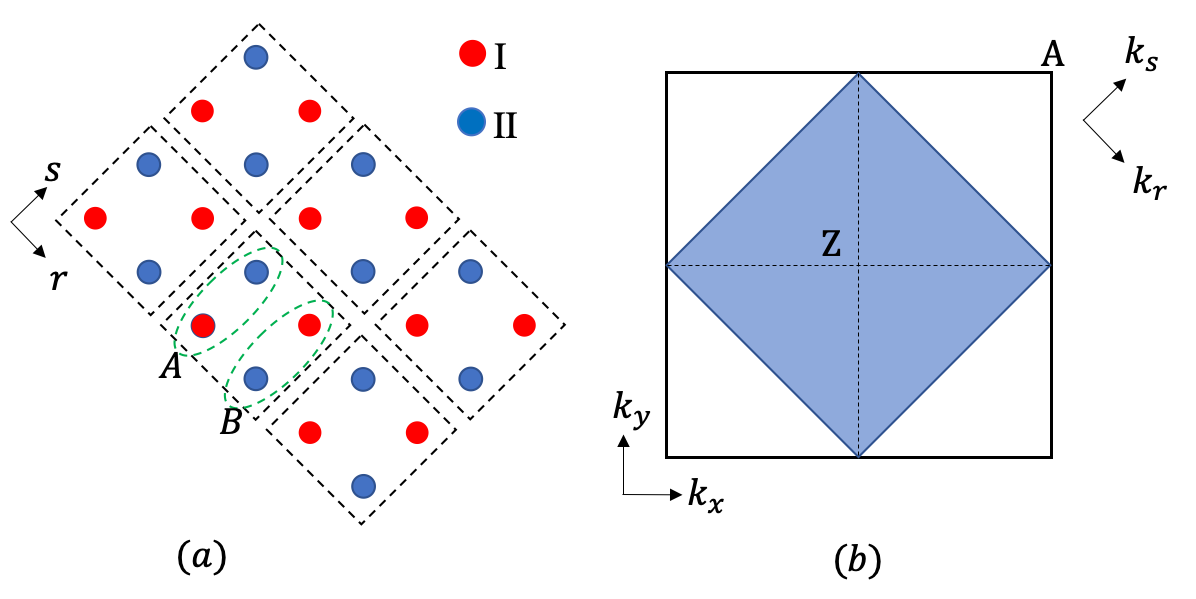
\includegraphics[width=\textwidth]{enlarged.png}
    \caption{(a) The enlarged unit cell(doted black box) with new sublattice indices $\sigma = A, B$ and rotated coordinates $r$ and $s$. (b) Enlarging the unit cell in XY plane has the effect of doubling the area of the unit cell in real space, which in turns reduce the area of the $k_x k_y$ plane in the Brillouin Zone by half.The outer square is the BZ for orginal unit cell. The shaded blue square is the BZ for enlarged unit cell}\label{fig:enlarged}
\end{figure}
The real space tight binding model above realizes the Weyl energy spectrum in the low energy regime when Fourier transformed to $k$-space, with the high symmetry Weyl points $Z = (0, 0, \frac{\pi}{c})$ and $A = (\frac{\pi}{a}, \frac{\pi}{a}, \frac{\pi}{c})$ shown in Fig \ref{fig:enlarged}(b). Expanding near the Weyl points, the $k \cdot p$ Hamiltonian reads
\begin{eqnarray}
    H ( Z + \delta \mathbf{k}) &=& (-\hbar v + c u_1 + c \tilde{u_1} ) \delta k_z \tau_y + u_2 a^2 \delta k_x \delta k_y \tau_z \mu_z \nonumber \\ &+& \frac{1}{2} a^2 (\tilde{u_1} - u_1) (\delta k_x^2 - \delta k_y^2) \tau_x \mu_z , \\  
    H (A + \delta \mathbf{k}) &=& (-\hbar v - c u_1 -c \tilde{u_1}) \delta k_z \tau_y + u_2 a^2 \delta k_x \delta k_y \tau_z \mu_z \nonumber \\ &-& \frac{1}{2} a^2 (\tilde{u_1} - u_1)(\delta k_x^2 - \delta k_y^2) \tau_x \mu_z .
\end{eqnarray}
Integrating the Berry curvature around the surface $\partial V$ enclosing the Weyl points in 3D Brillouin Zone
\begin{equation}
\mathcal{C} = \frac{1}{2\pi}\int_{\partial V} d^3 \mathbf{k} \nabla_{\mathbf{k}} \times \bra{\psi (\mathbf{k})}  \ket{\nabla_{\mathbf{k}} \psi (\mathbf{k})} ,
\end{equation}
 gives us four quadratic Weyl points with Chern number $\mathcal{C} =-8$ at the $Z$ point and another four with opposite Chern number $\mathcal{C} =+8$ at the $A$ point.

The distinctive topological Fermi-arc surface states are a prominent feature of Weyl semimetals. In order to verify the existence of such surface states in (TaSe4)2I, Shi*, W., Wieder*, B.J., Meyerheim*, H.L. et al\cite{shi2021charge} employed surface Green's functions to compute the surface states. In (001)-surface, we can see clear surface states at the center and corner of BZ, which matches with our $k\cdot p$ Hamitonian. Our model captured  topological features for Weyl semimetalic phase of (TaSe4)2I.

\begin{figure}[h]
    \centering
    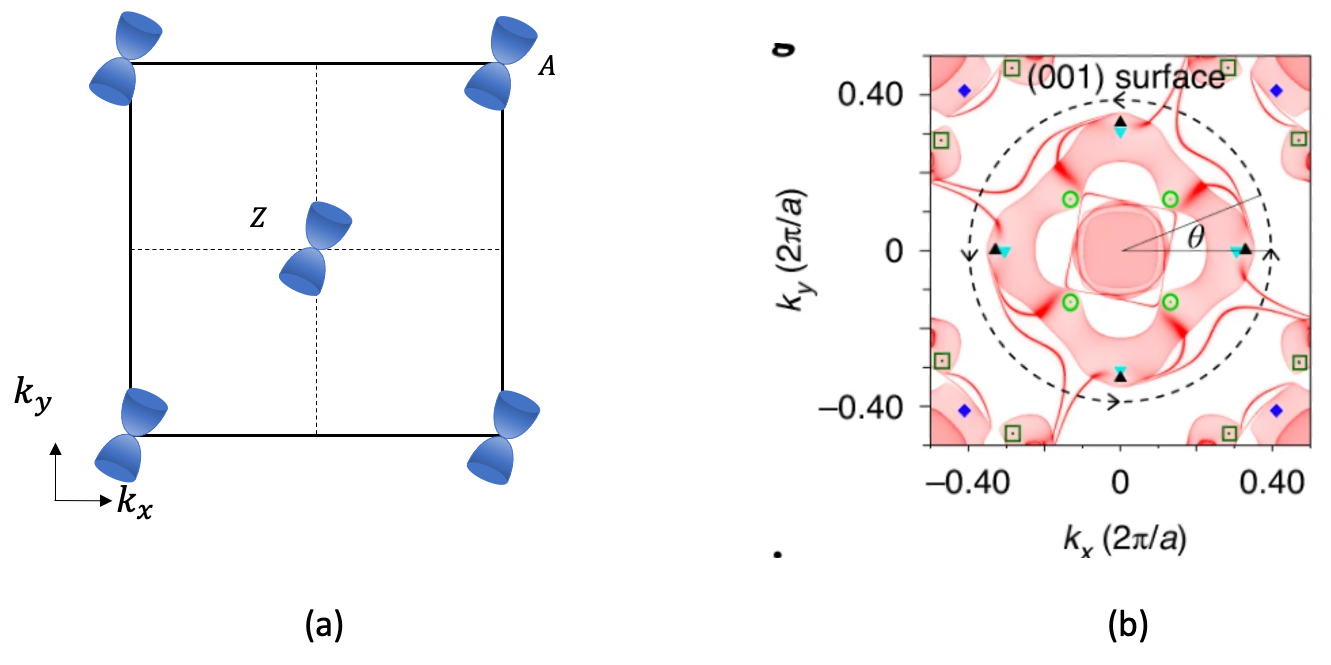
\includegraphics[width=\textwidth]{images/Weyl_points.png}
    \caption{A comparision between $k\cdot p$ Hamiltonian and DFT, showing our model captured all topological features of DFT calculation. (a) Quadratic Weyl points in BZ at $k_z=\frac{\pi}{c}$ from our $k\cdot p$ Hamiltonian. (b) DFT calculation shows the surface states of $($TaSe$_4)_2$I terminated in the experimentally favoured (001) direction. The projected Fermi pockets shows Chern number equals to 8 at the corner and center of the surface Brillium zone \cite{shi2021charge}.}
    \label{fig:weyl_points}
\end{figure}


The Weyl points are protected by the symmetries. In a spinless model, $C_{2x}$ and $C_{4z}$ generate the the point group $C_{4v}$ . Their operator representations and character table are shown in Table (\ref{C4vsymmTRIM}) and (\ref{C4spinlessCharacterTable}) respectively. The fourfold degeneracy at $Z$ decomposes into the $D_8$ representations $\tilde{\rho}_Z=A_1\oplus A_2\oplus B_1\oplus B_2\label{spinlessrepZ}$ while at $A$ point it decomposes into $\tilde{\rho}_A=E\oplus E$.

\begin{table}[h]
\begin{tabular}{c|cc}
&Z&A\\
\hline
$\tilde{C}_{2x}$&$\tau_x$&$\tau_x\mu_z$\\
$\tilde{C}_{4z}$&$\mu_x$&$-i\mu_y$
\end{tabular}.
\caption{The rotation operator representations at $Z$ and $A$ points.} \label{C4vsymmTRIM}
\end{table}

 \begin{table}[h]
 \begin{tabular}{c|ccccc}
 &[1]&[$C_{4z}^2$]&[$C_{2x}$]&[$C_{2xy}$]&[$C_{4z}$]\\
 \hline 
 $A_1$&1&1&1&1&1\\
 $A_2$&1&1&-1&-1&1\\
 $B_1$&1&1&1&-1&-1\\
 $B_2$&1&1&-1&1&-1\\
 $E$&2&-2&0&0&0
 \end{tabular}
 \caption{The character table for the point group $C_{4v}$.} \label{C4spinlessCharacterTable}
 \end{table}

{\color{red} No folding} 
The density wave breaks the $\hat{T}_{1/2}$ symmetry and enlarge the unit cell in Fig \ref{fig:enlarged}. Intuitively, the Weyl points with different Chern number at $Z$ and $A$ will be folded together and we can add mass term M in the enlarged unit cell
\begin{equation}
    H= \begin{bmatrix}
    H_Z & M \\
    M^\dagger & H_A 
    \end{bmatrix}.
\end{equation}
It has to satisfy the symmetry constraints
\begin{equation}
    \begin{bmatrix}
    \hat{\rho}_Z & 0 \\
    0 & \hat{\rho}_A 
    \end{bmatrix}\begin{bmatrix}
    0 & M \\
    M^\dagger & 0 
    \end{bmatrix}
    \begin{bmatrix}
    \hat{\rho}_Z^{-1} & 0 \\
    0 & \hat{\rho}_A^{-1} 
    \end{bmatrix}
    =
    \begin{bmatrix}
    0 & M \\
    M^\dagger & 0 
    \end{bmatrix} ,
\end{equation}
which leads to $\hat{\rho}_Z=M\hat{\rho}_AM^{-1}$. However, taking trace on this equation will give $\mathrm{Tr}(\hat{\rho}_Z) = \mathrm{Tr}(\hat{\rho}_A)$, which contradicts with the $C_{4v}$ representation ({\color{red} unclear, need more elaboration}). Therefore, the Weyl points are robust against $\hat{T}_{1/2}$ breaking terms in spinless model while preserving other symmetries. We have to introduce SOC to gap this Weyl semimetal phase. 

\begin{table}[h]
\begin{tabular}{c|ccccccc}
   &[1]&[C_{4z}^2]&[C_{2x}]&[C_{2xy}]&[C_{4z}]&[-1]&[-C_{4z}]\\\hline
A_1&1&1&1&1&1&1&1\\
A_2&1&1&-1&-1&1&1&1\\
B_1&1&1&1&-1&-1&1&-1\\
B_2&1&1&-1&1&-1&1&-1\\
E&2&-2&0&0&0&2&0\\
E_{1/2}&2&0&0&0&\sqrt{2}&-2&-\sqrt{2}\\
E_{-1/2}&2&0&0&0&-\sqrt{2}&-2&\sqrt{2}%\\E_{3/2}&4&0&0&0&0&-4&0
\end{tabular}\label{ChtableD4h}
\caption{Double group character table for the group $C_{4v}$.}
\end{table}


\begin{table}[h]
\begin{tabular}{c|cc}
  &Z&A\\\hline 
C_{2x} & $is_x\tau_x$ & $is_x\tau_x\mu_z$ \\
C_{4z} & $e^{i(\pi/4)s_z}\mu_x$ & $-ie^{i(\pi/4)s_z}\mu_y$
\end{tabular}\label{D4hsymmTRIM}
\caption{Symmetry representations with SOC.}
\end{table}


The spinful double group of $C_{4v}$ includes another $2\pi$ rotation to the group of $C_{4v}$. Its character table and representations are given in (\ref{ChtableD4h}) and (\ref{D4hsymmTRIM}). The model is doubled and the eightfold  degeneracy at the $\mathrm{Z}$ and $\mathrm{A}$ points decompose into $\rho_\mathrm{Z} = \rho_\mathrm{A} =E_{1/2}\oplus E_{-1/2}\oplus E_{1/2}\oplus E_{-1/2}$ respectively. 
It is then possible to add mass terms and gap Weyl semimetal into different topological phases. 


%The symmetry operators (present argument from section 2.2 and 2.3 in TaSe file. Write spinful symmetry operator in k space and then k dot p? Ask Meng)(Be sure to highlight why spinful case is needed for CDW gapping, from irreducible rep point of view)

% Switch to spinful case, describe the irreducible representations.



%\begin{itemize}
%    \item Tight-binding model Hamiltonian
%    \item kp description of Weyl semimetal without SOC %(robust Weyl points)
%    \item gapping terms with SOC and different 3D topological phases
%    \item vortex
%    \item k-theory of defect
%\end{itemize}

%(Show that with C4, you can use 2C to read off the answer for a hypothetical $Q = (\pi,\pi,0)$ C4-symmetric (bidirectional) CDW, and 2D to read off the answer for the more realistic unidirectional $(pi,pi,0)$ CDW.)

% Rewrite the tight-binding model and k.p Hamiltonian in the enlarged unit cell => Dirac semimetal protected by symmetry in the spinless case because the representations at Z and A are different. => Dirac mass has to be spin-orbit coupled



% \section{electron scattering}

% In 1961, Robert Hofstadter wins Nobel Price for his pioneering studies of structure of nucleons with  electron scattering. Accelerated electron beams are widely used for study the inner structure of the nucleons (and neutrons) since then. Those experiment can provide different level structure information of nucleons given different incident electron energy. At the range where the energy of electrons are very low, $\lambda \gg r_p$, here $r_p$ is the radius of the proton, $\lambda$ is the electron wavelength, the scattering is equivalent to scattered over point like spin-less object. At low electron energy range where $\lambda ~r_p$, the scattering is equivalent to scattering over charged object. When the electron wavelength $\lambda < r_p$, the electron scattering will be able to see the substructures. At very high energy range where $\lambda \ll r_p$, the electrons is equivalent to scattering over the sea of quarks and gluons of the protons. 

% In one photon exchange approximation, the  transition current for nucleon can be write as:

% $$
% J^\mu = e\bar{\mu}\Gamma^\mu(p)e^{i\vec{q}\vec{x}}$$
% $$

% \todo[inline]{Add the Feynman diagram}

% In one photon exchange approximation, the cross section of electron scattered over spin-0 particle would be:

% $$
% \frac{d\sigma}{d\Omega} = \frac{d\sigma}{d\Omega}|F(Q^2)|
% $$

% \todo[inline]{current result of proton radius (PRad)}

% \subsection{e-p scattering with exchange of photon}
% \subsection{weak interation with exchange of $Z^0$ Boson}
% \subsection{form factor}


% \section{Parity Violation}
% \section{Parity Violation Asymmetry}
% \section{Rich Physics Behind the PRex Experiment}
% \subsection{EOS of Neutron rich matter}